\documentclass{beamer}
\usepackage[utf8]{inputenc}
\usepackage{multicol}
\usepackage{amsmath}
\usepackage[english]{babel}

\begin{document}

\begin{frame}
\frametitle{Problema 1}
 Demuestren que la solucion dada para cada recurrencia es la correcta utilizando el método de sustitutción.
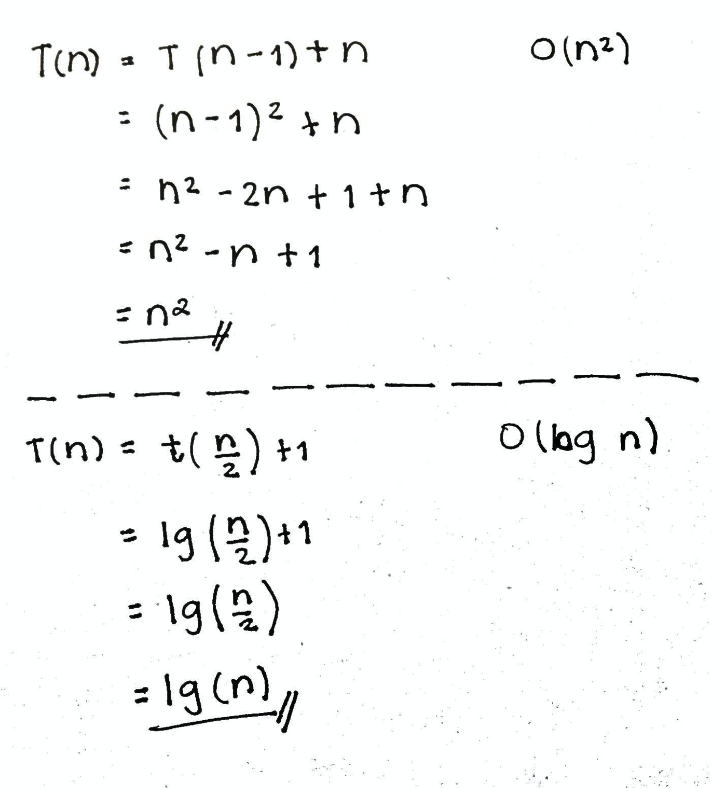
\includegraphics[width=6cm]{p1.png}

\end{frame}

\begin{frame}
\frametitle{Problema 2}
Utilicen el metodo de arbol recursivo para encontrar un limite asintotico. Utilicen el metodo de sustitucion para comprobar.
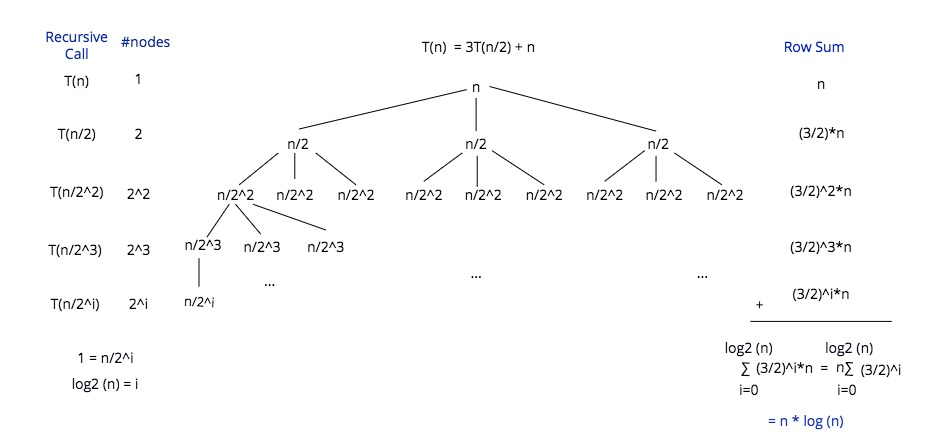
\includegraphics[width=12cm]{p2.jpg}

\end{frame}
\begin{frame}
 Utilicen el metodo de sustitucion para comprobar.
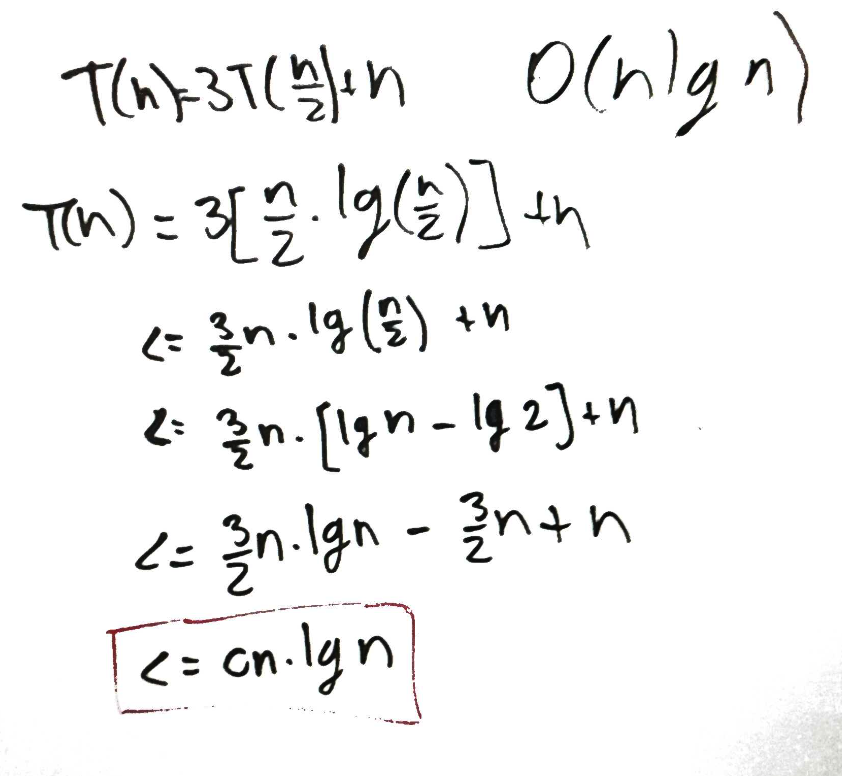
\includegraphics[width=8cm]{p2_2.png}

\end{frame}

\begin{frame}
\frametitle{Problema 3}
Encuentren un limite asintotico para cada problema utilizando el metodo maestro.
\newline
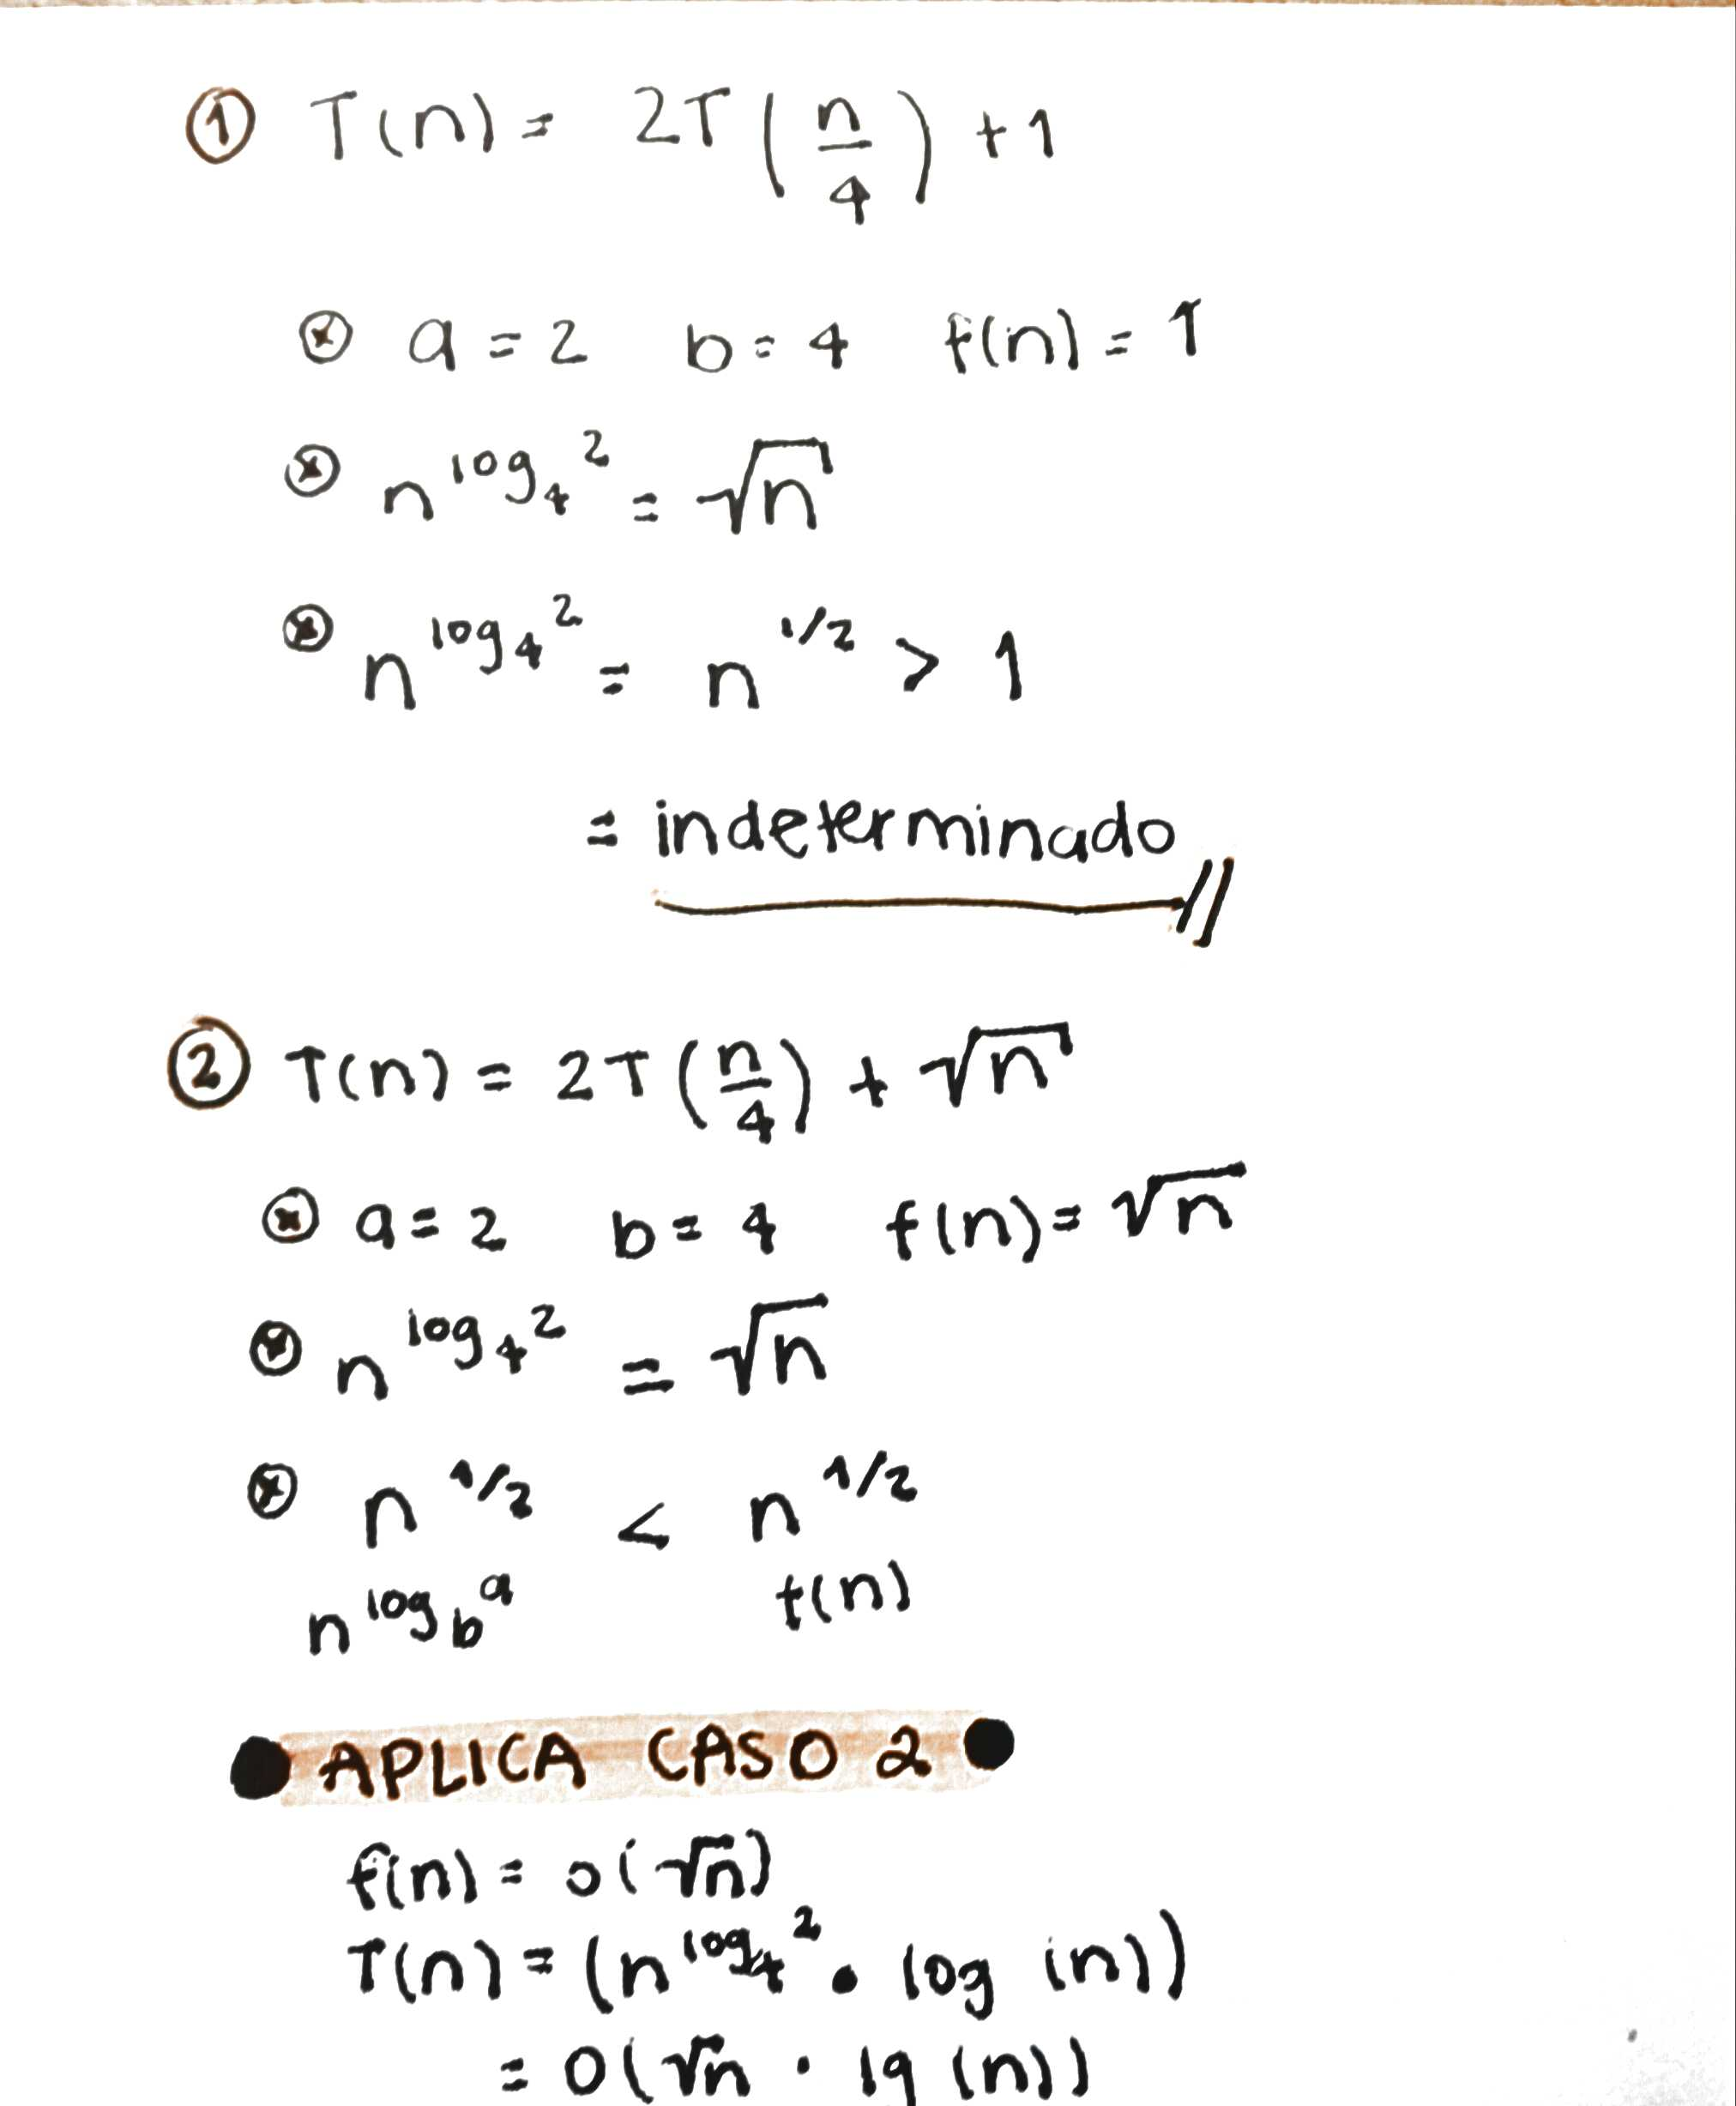
\includegraphics[width=6cm]{1.jpg}
\end{frame}
\begin{frame}
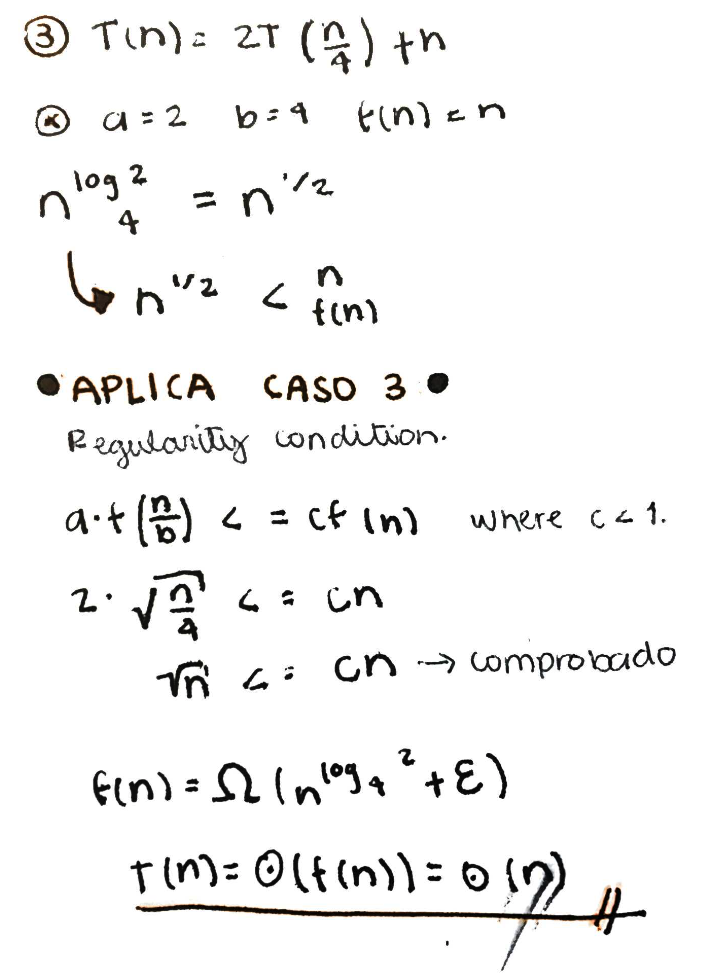
\includegraphics[width=6cm]{3.png}
\end{frame}
\begin{frame}
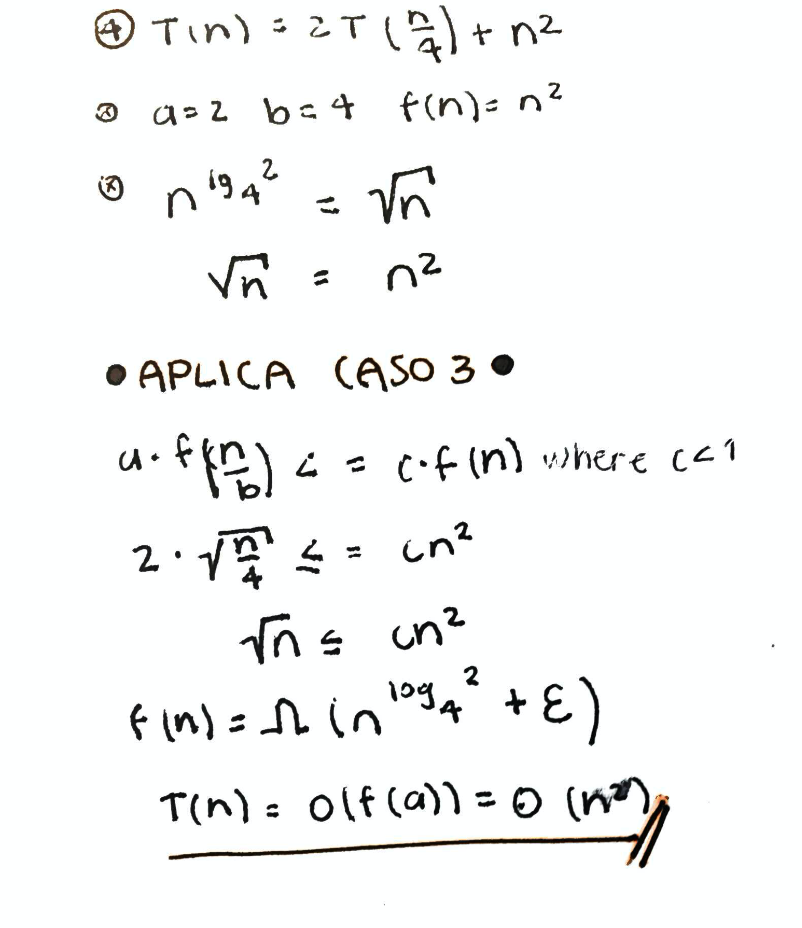
\includegraphics[width=7cm]{4.png}

\end{frame}
\end{document}

